%%
%% Copyright 2021 OXFORD UNIVERSITY PRESS
%%
%% This file is part of the 'pnas-nexus-authoring-template Bundle'.
%% ---------------------------------------------
%%
%% It may be distributed under the conditions of the LaTeX Project Public
%% License, either version 1.2 of this license or (at your option) any
%% later version.  The latest version of this license is in
%%    http://www.latex-project.org/lppl.txt
%% and version 1.2 or later is part of all distributions of LaTeX
%% version 1999/12/01 or later.
%%
%% The list of all files belonging to the 'pnas-nexus-authoring-template Bundle' is
%% given in the file `manifest.txt'.
%%
%% with bibliographic references
%%

\documentclass[unnumsec,webpdf,contemporary,large]{Article}%

%\usepackage{showframe}

\graphicspath{{images/}}

% line numbers
%\usepackage[mathlines, switch]{lineno}
%\usepackage[right]{lineno}

\theoremstyle{thmstyleone}%
\newtheorem{theorem}{Theorem}%  meant for continuous numbers
%%\newtheorem{theorem}{Theorem}[section]% meant for sectionwise numbers
%% optional argument [theorem] produces theorem numbering sequence instead of independent numbers for Proposition
\newtheorem{proposition}[theorem]{Proposition}%
%%\newtheorem{proposition}{Proposition}% to get separate numbers for theorem and proposition etc.
\theoremstyle{thmstyletwo}%
\newtheorem{example}{Example}%
\newtheorem{remark}{Remark}%
\theoremstyle{thmstylethree}%
\newtheorem{definition}{Definition}


\begin{document}

\copyrightyear{2022}
\appnotes{~}

\firstpage{1}

%\subtitle{Subject Section}

\title[Regression, Chess as a Model System]{Performing Regression on Complex Data using a
Squeeze-and-Excitation Residual Neural Network, Chess as a Model System}

\author[a]{Gaëtan Serré}

\corresp[a]{\href{mailto:gaetan.serre@universite-paris-saclay.fr}{gaetan.serre@universite-paris-saclay.fr}}

\authormark{Gaëtan Serré}


\received{Date}{0}{Year}
\accepted{Date}{0}{Year}

%\editor{Associate Editor: Name}

\abstract{
  As neural networks for image recognition become more and more powerful
  and AI becomes more and more present in all fields,
  it would be very helpful to be able to use these models
  with non-image data and get good performance.
  This paper aims to show that this is possible through an model system very
  related to artificial intelligence: chess.\\
  We can simplify a chess engine in two main components: an evaluation function,
  which is a function that takes a chess position as input and returns a score 
  and a search algorithm which will uses the evaluation function to find the best move
  to play in a given position.\\
  I introduce GAiA, a chess engine which uses a Squeeze-and-Excitation
  residual network as an evaluation function. GAiA's neural network
  try to reproduce the evaluation function of a world reknown chess engine.
  With only few hours of training, GAiA's neural network has
  an accuracy of 0.93 (using the coefficient of determination).\\
  These results suggest that Squeeze-and-Excitation residual networks,
  which are the state-of-the-art neural networks for image recognition,
  can be used with data that are not images.
}
\keywords{Artificial Intelligence, Deep Learning, Neural Networks, Chess}

%\boxedtext{
% Research reports require a significance statement of between 50 and 120 words. Abbreviations are permitted, but citations cannot be included. If required, un-comment this element in the template to include. The heading is included automatically.
%}

\maketitle
\section{Introduction}

Artificial intelligence for image recognition is becoming
increasingly powerful. Since 2015, thanks to the ResNet\cite{resnet}
architecture, we achieve astounding performance on the ImageNet database.
Furthermore, in 2017 is introduced Squeeze-and-Excitation\cite{squeezeandexcitation}
network architecture which significantly
improve the performance of ResNet with almost no additional computation costs.

The question is: can we use this architecture on data that are not
originally images. If so, we just have to encode our data in 3-dimensional
tensors and look for the number of Squeeze-and-Excitation residual
blocks (Figure \ref{fig:seblock}) and other hyperparameters
that optimizes our results to get excellent performance.
The challenge is to know if Squeeze-and-Excitation networks are
generalizable to any kind of machine learning problem.

As a chess fan, I have chosen to show that it was possible to create a
high-performance chess engine using this type of neural network.
I have called this chess engine GAiA.

\begin{figure}[H]
  \centering
  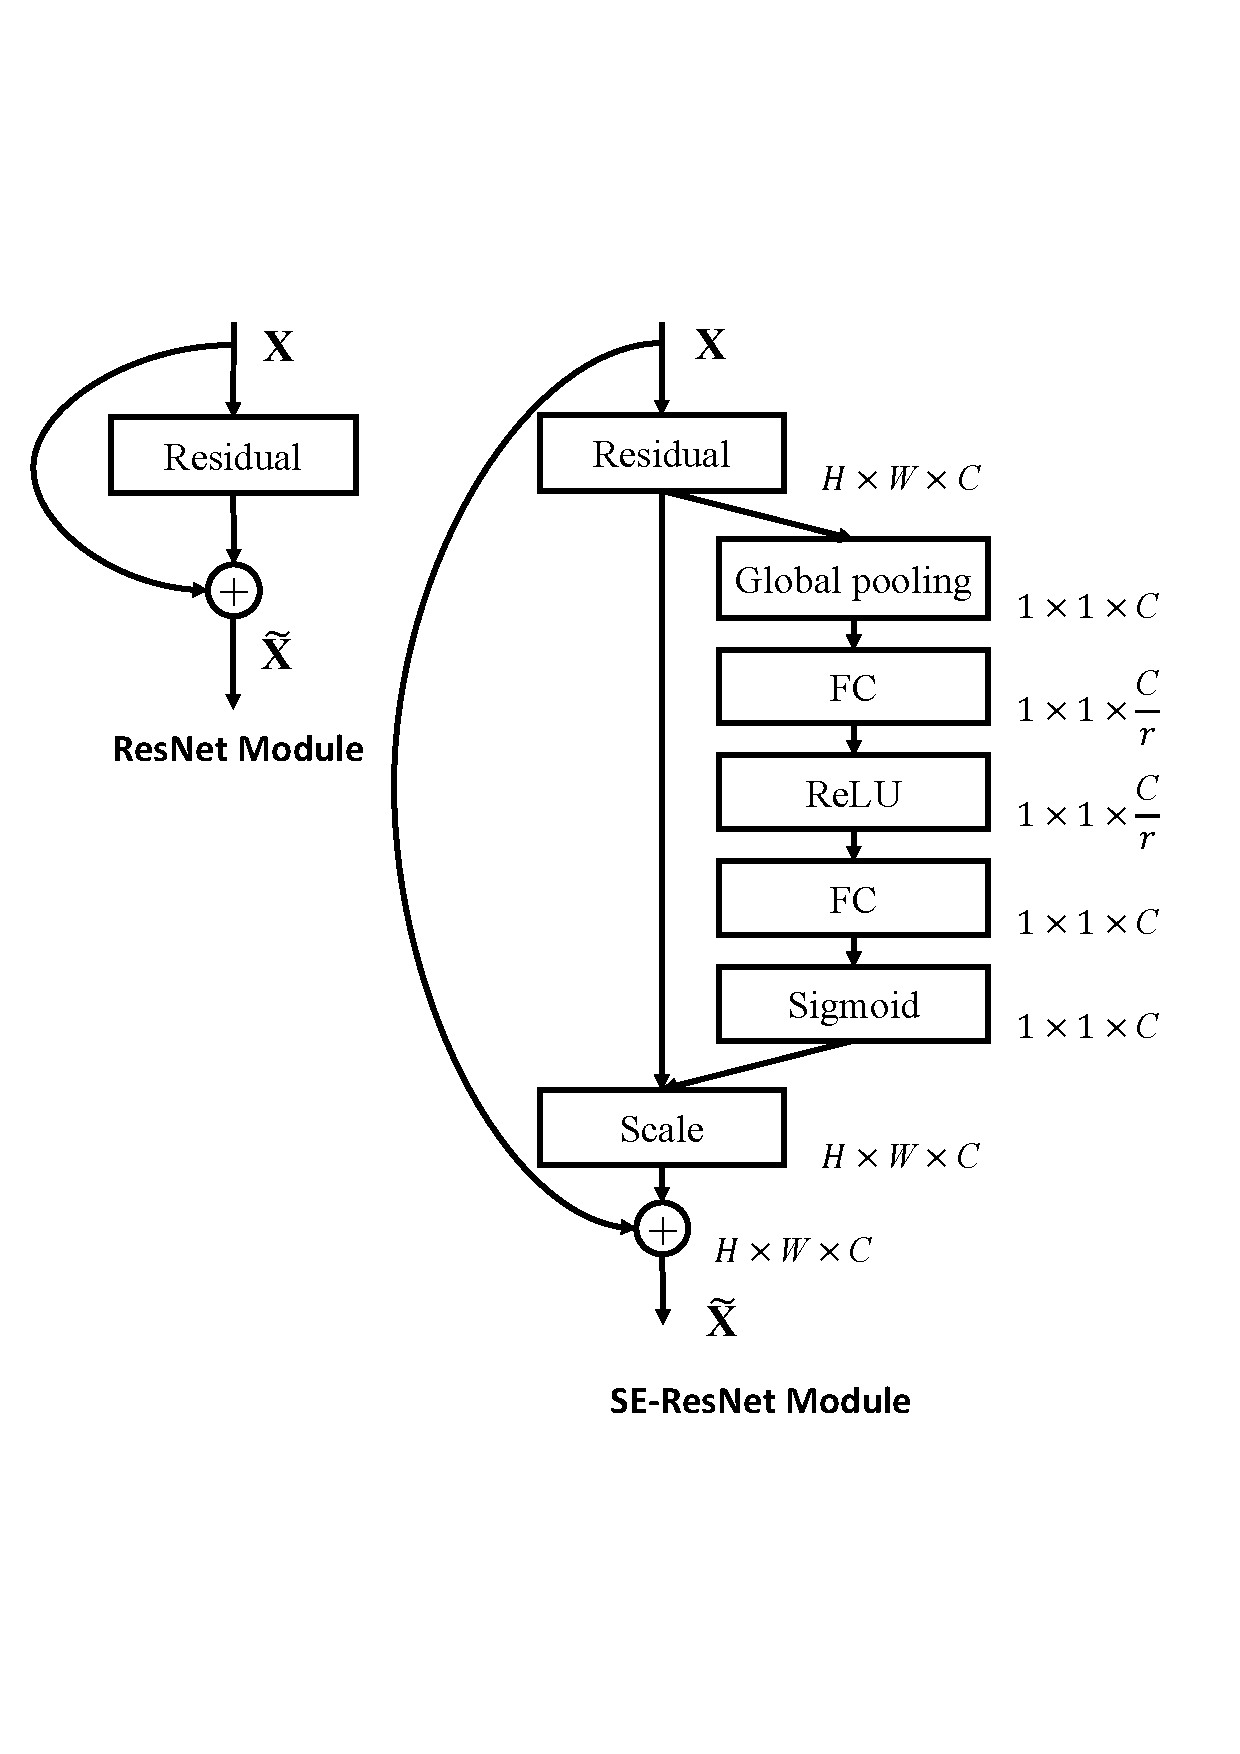
\includegraphics[width=7cm]{module_seresnet.pdf}
  \caption{The schema of the original Residual block (left) and the SE-ResNet
  block (right)}
  \label{fig:seblock}
\end{figure}


\section{Data}
GAiA's neural network tries to recreate the evaluation function of Stockfish 14\cite{stockfish},
a open-source world reknown chess engine. It uses heuristics function written
by human experts to evaluate position. Stockfish also uses a classical
alpha-beta game tree search with plenty optimizations to find the best move.
GAiA is a combination of the Stockfish game tree search algorithm and a
Squeeze-and-Excitation residual network as evaluation function.

In order to train GAiA's neural network, I needed tons of different
chess position. Lichess.org\cite{lichess} is a popular, free and open-source
chess platform which provides millions of games played by humans every month.
From these games, I extracted millions of different positions along with their
Stockfish 14 evaluation. If we look at the distribution of the evaluations
(Figure \ref{fig:distribution}), we can see that the overwhelming majority
is close to $0$ i.e draw game.
Each position is encoded as a $8\times8$ image with $15$ channels: 
$12$ representing each chess pieces, $1$ for the actual player, $1$
for the en-passant square and $1$ for the castling rights.


\begin{figure}[H]
  \captionsetup[subfigure]{labelformat=empty}
  \centering
  \subfloat[]{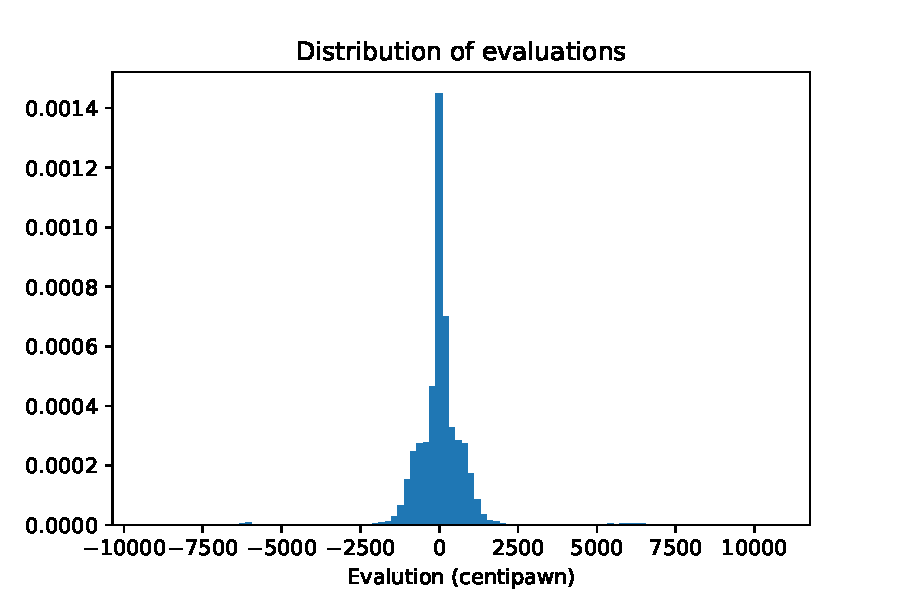
\includegraphics[width=3.1in]{distribution.pdf}}\\
  \subfloat[]{
    \begin{tabular}{ | l | c | }
      \hline
      count & 1,389,333 \\ \hline
      mean  & 30.14 \\ \hline
      std   & 942.35\\ \hline
      min   & 9873\\ \hline
      25\%  & -254.0\\ \hline
      50\%  & 28.0\\ \hline
      75\%  & 320.0\\ \hline
      max   & 13,678.0\\ \hline
    \end{tabular}
  }
  \caption{Distribution of the evaluations}
  \label{fig:distribution}
\end{figure}


\section{Neural Network Structure}
GAiA's model architecture is composed of $4$ SE-ResNet blocks of $2$ convolutional layers
each with $64$ filters and a kernel shape of $1\times1$ using \textit{ReLU} activation function.
To find these hyperparameters, I tried several values and these ones seemed to be
the best compromise between computation costs and accuracy.
(Figure \ref{fig:acc_loss} \& \ref{fig:score_valid})
The output is a fully connected layer using \textit{Linear} readout function (Figure \ref{fig:model_archi}).
This model architecture is designed based on Maia\cite{maia}.
The loss is the Mean Absolute Error and the accuracy the coefficient of determination.
I used the framework Tensorflow 2.7\cite{tensorflow} to create and train the neural network.
The model is trained on $\sim 1,400k$ positions and tested on $\sim 400k$
during 30 epochs (Figure \ref{fig:history}).

\begin{figure}[H]
  \captionsetup[subfigure]{labelformat=empty}
  \centering
  \subfloat[Loss]{
    \centering
    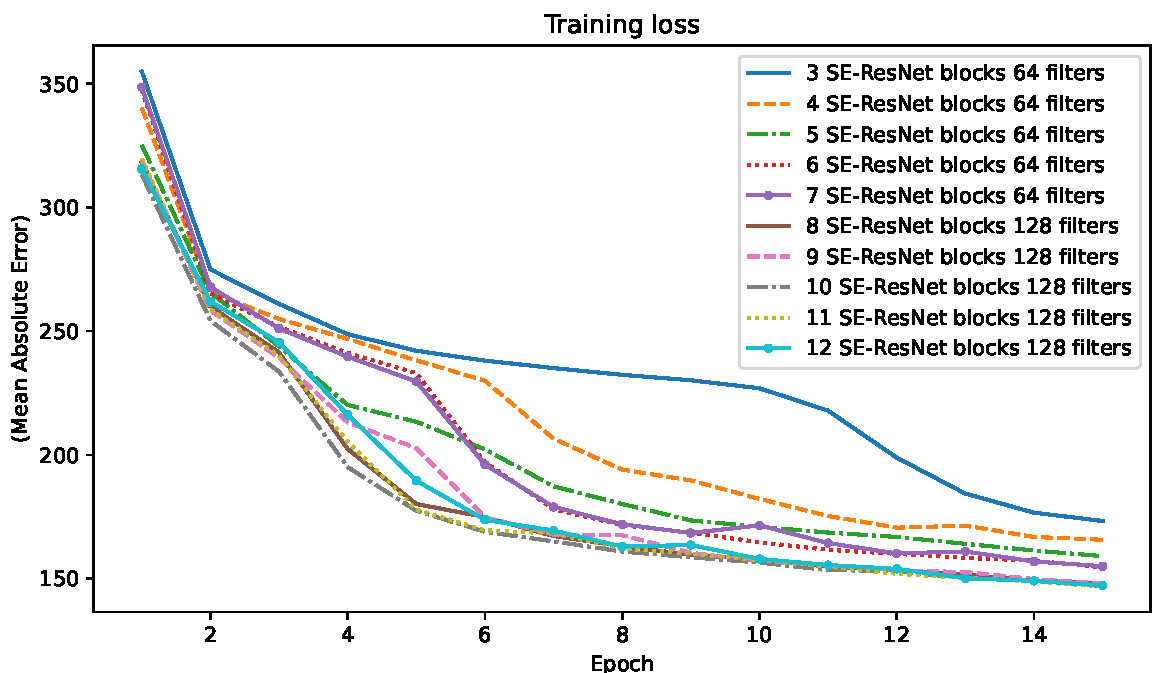
\includegraphics[width=8cm]{model_selection_1_loss.pdf}
  }\\
  \subfloat[Accuracy]{
    \centering
    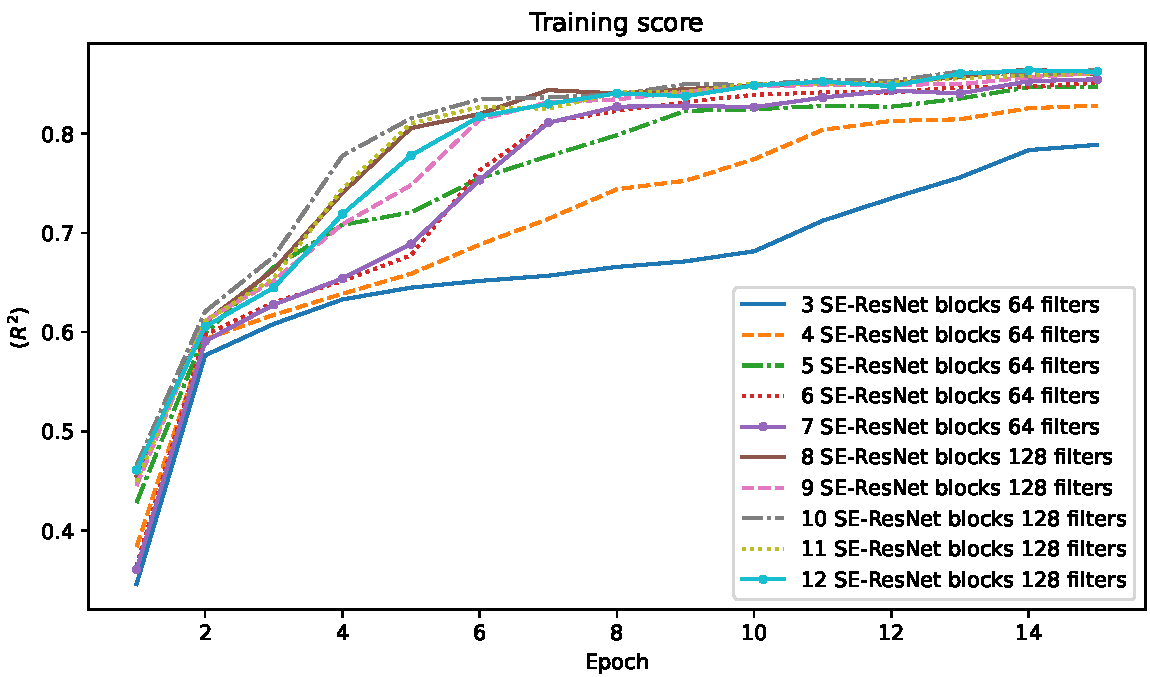
\includegraphics[width=8cm]{model_selection_1_score.pdf}
  }
  \caption{Loss and accuracy on train sets}
  \label{fig:acc_loss}
\end{figure}

\begin{figure}[H]
  \centering
  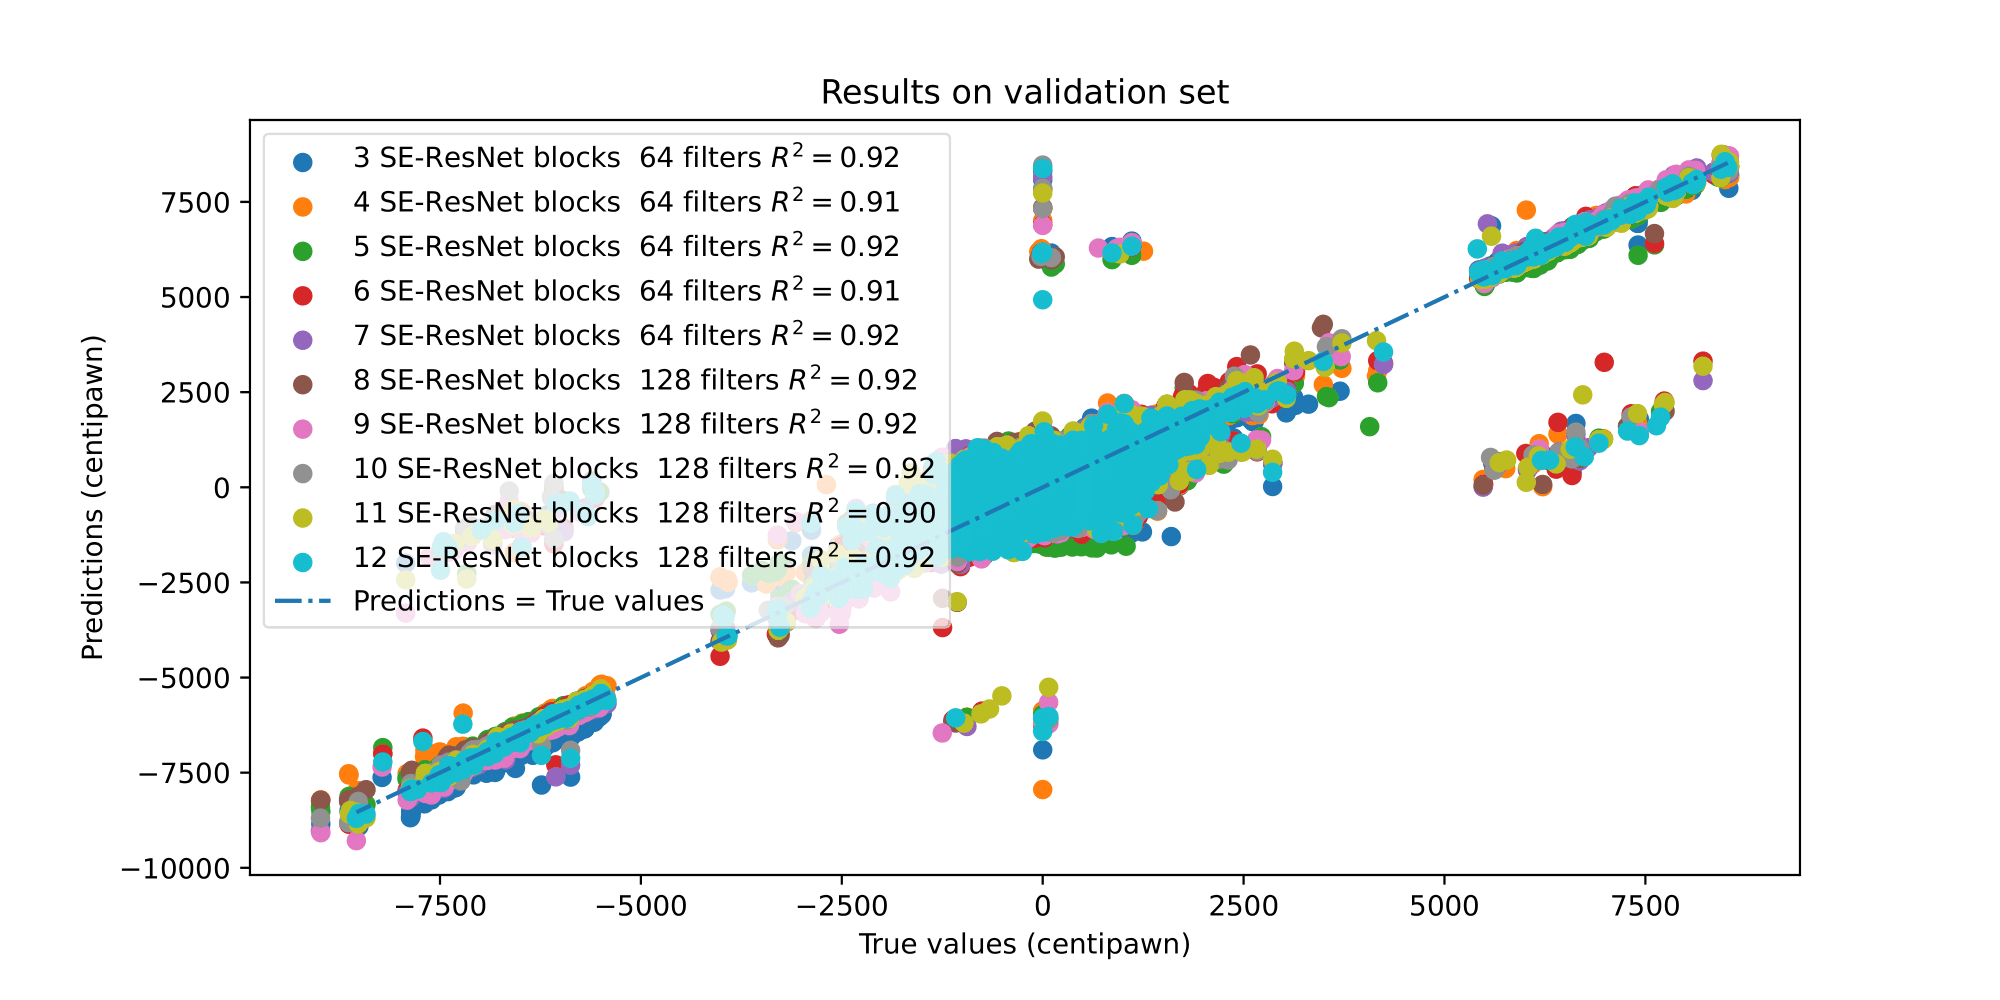
\includegraphics[width=10cm]{model_selection_2.png}
  \caption{Score on validation sets}
  \label{fig:score_valid}
\end{figure}

\begin{figure}[H]
  \centering
  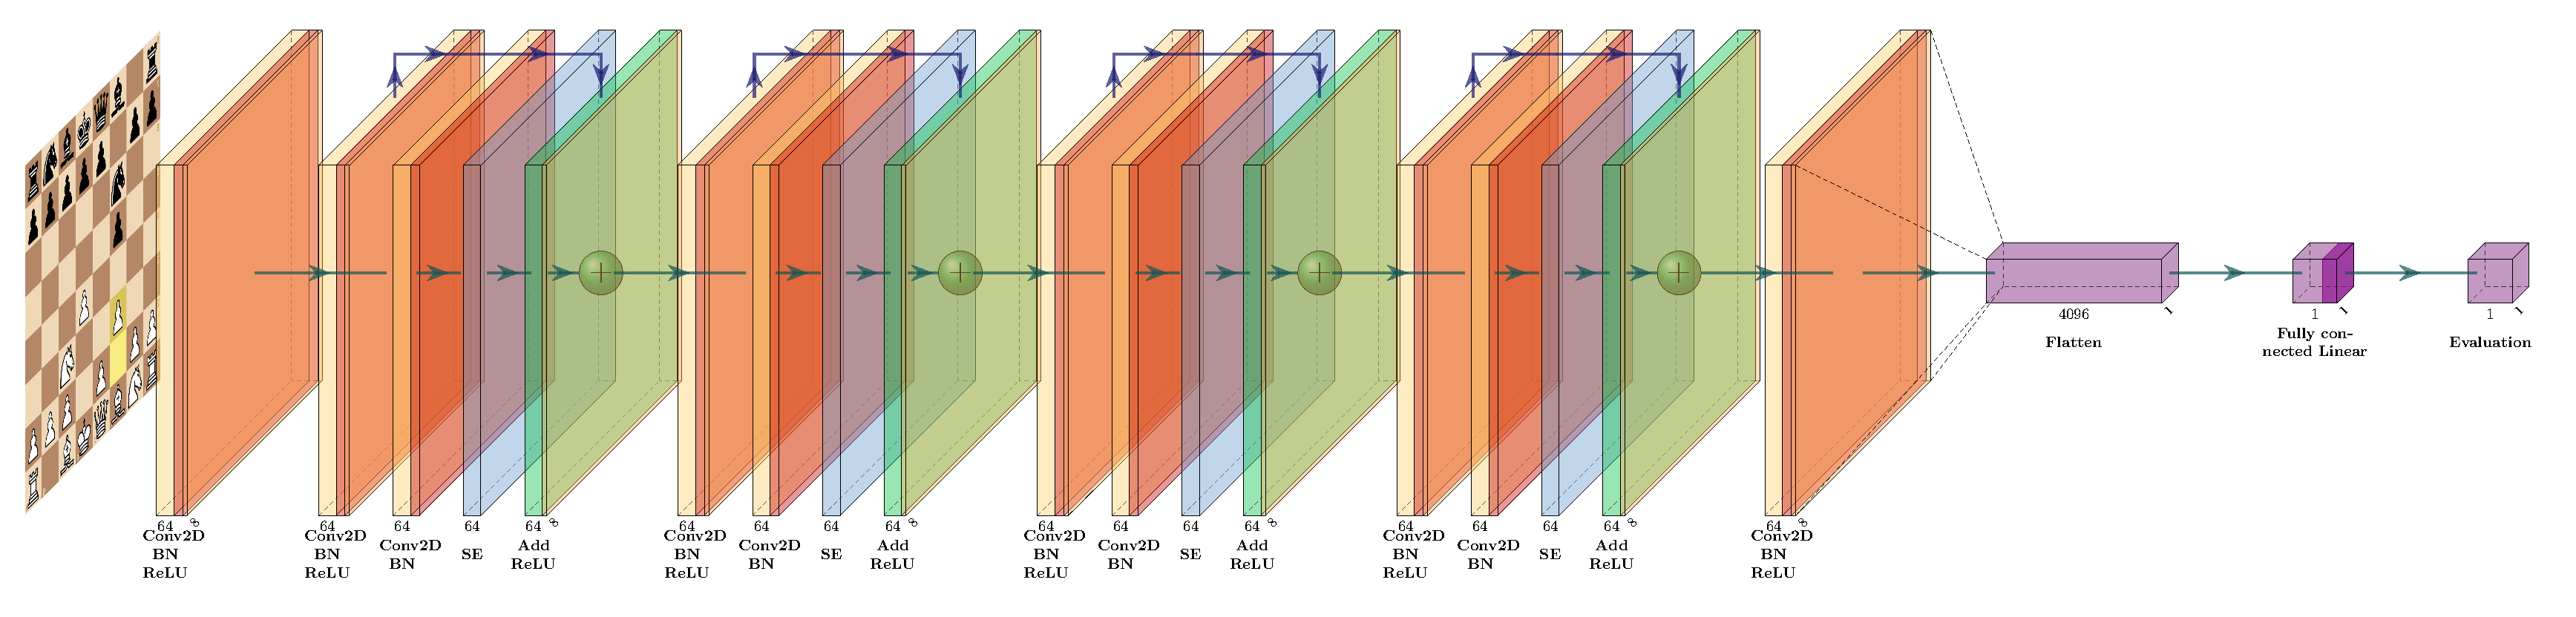
\includegraphics[width=9cm]{network/network.pdf}
  \caption{GAiA's neural network architecture}
  \label{fig:model_archi}
\end{figure}

\begin{figure}[H]
  \captionsetup[subfigure]{labelformat=empty}
  \centering
  \subfloat[Loss]{
    \centering
    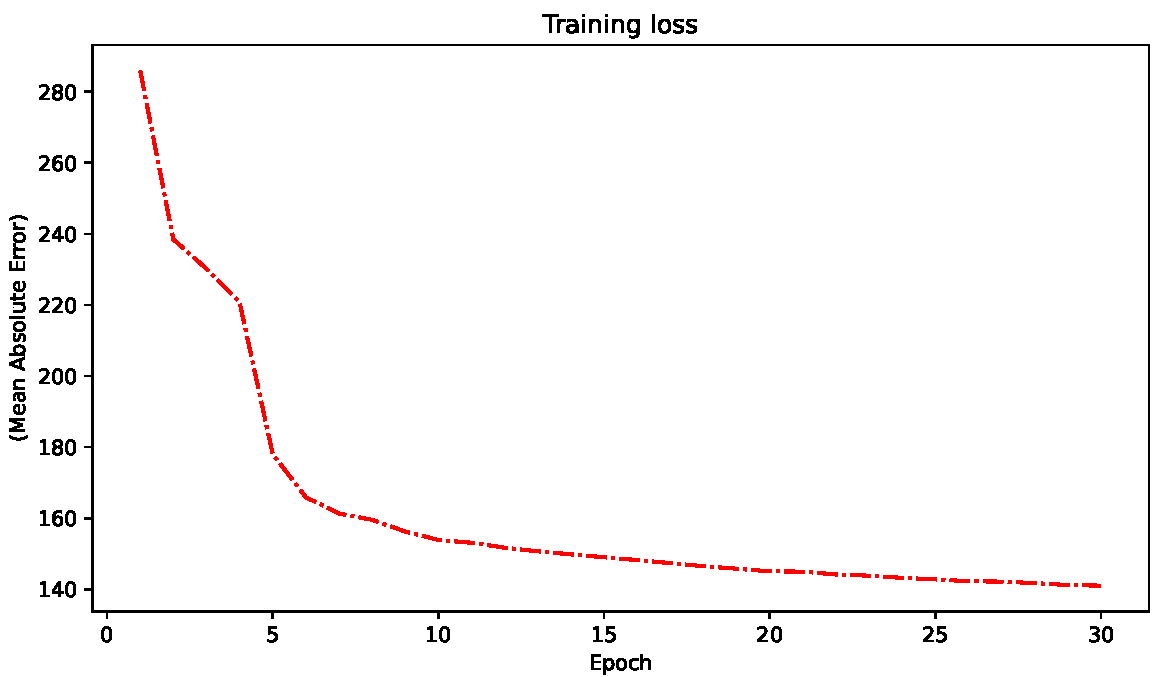
\includegraphics[width=8cm]{GAiA_history_loss.pdf}
  }\\
  \subfloat[Accuracy]{
    \centering
    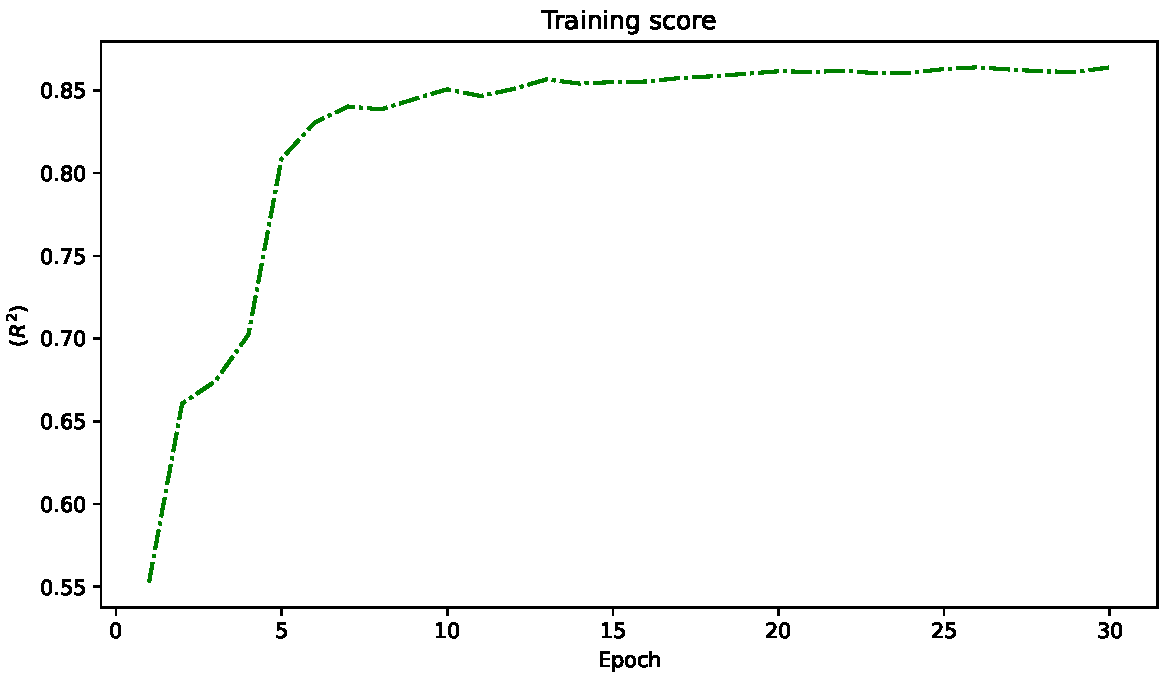
\includegraphics[width=8cm]{GAiA_history_score.pdf}
  }
  \caption{Loss and accuracy during training}
  \label{fig:history}
\end{figure}

\section{Results}
As we can see on the Figure \ref{fig:result}, GAiA's neural network
has great performance and I only trained it on $\sim 1,400k$ positions.
But some points are misplaced: these are positions where one of the kings is
in check. This is due to the fact that Stockfish cannot statically evaluate
position where a king is in check and so I had to search at depth $1$ (one move ahead).
The resulting evaluation takes into account the next move and therefore
is much more difficult to predict. However, the evaluations of
such positions produced by the network are not meaningless,
and are even quite close to a static evaluation of the position.
(Figure \ref{fig:misplaced})\\
Even if GAiA (the complete chess engine) can see much less positions
per second than "classic" chess engine (inferring an evaluation of a chessboard
from such a complex neural network is much more time consuming than
use heuristics functions), it has been able to defeat many engines
around 2000 elo on Lichess.org.

\begin{figure}[H]
  \centering
  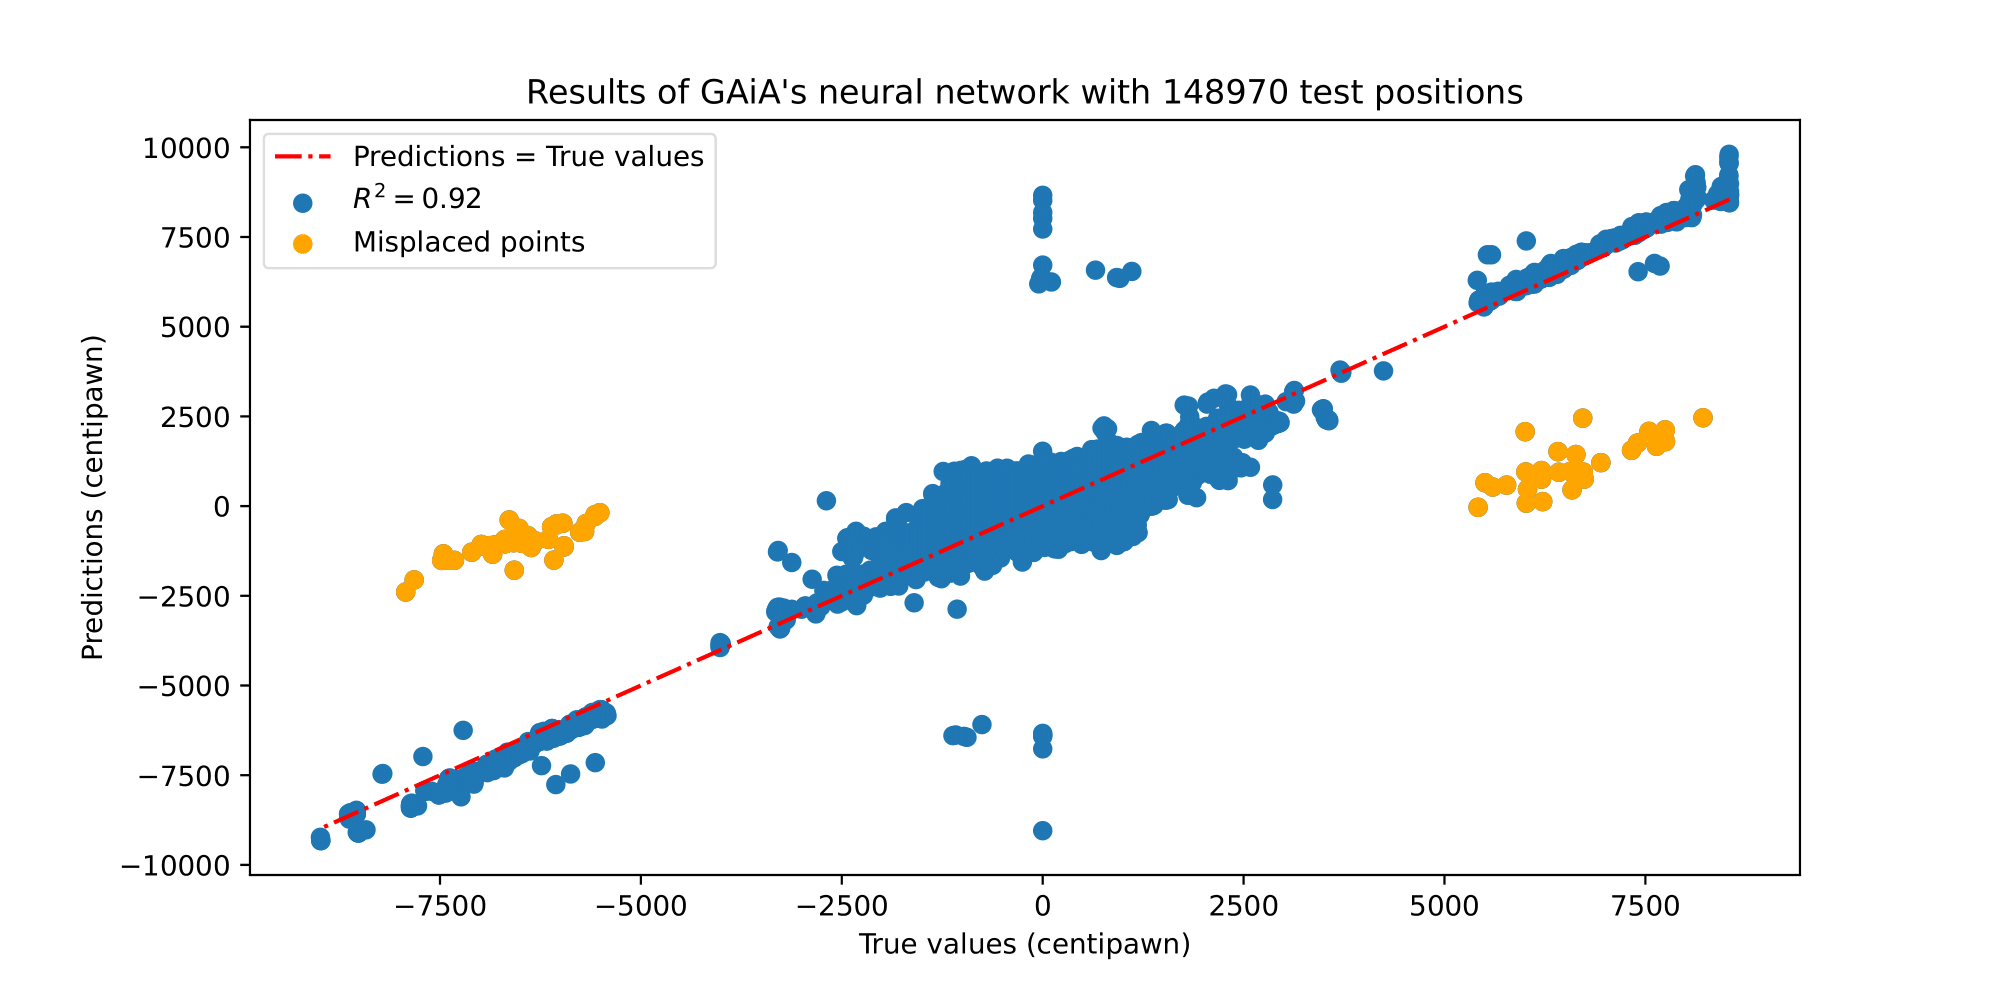
\includegraphics[width=8cm]{result.png}
  \caption{GAiA's neural network results}
  \label{fig:result}
\end{figure}

\begin{figure}[H]
  \captionsetup[subfigure]{labelformat=empty}
  \centering
  \subfloat[Stockfish score: 863, GAiA score: 6348]{
    \centering
    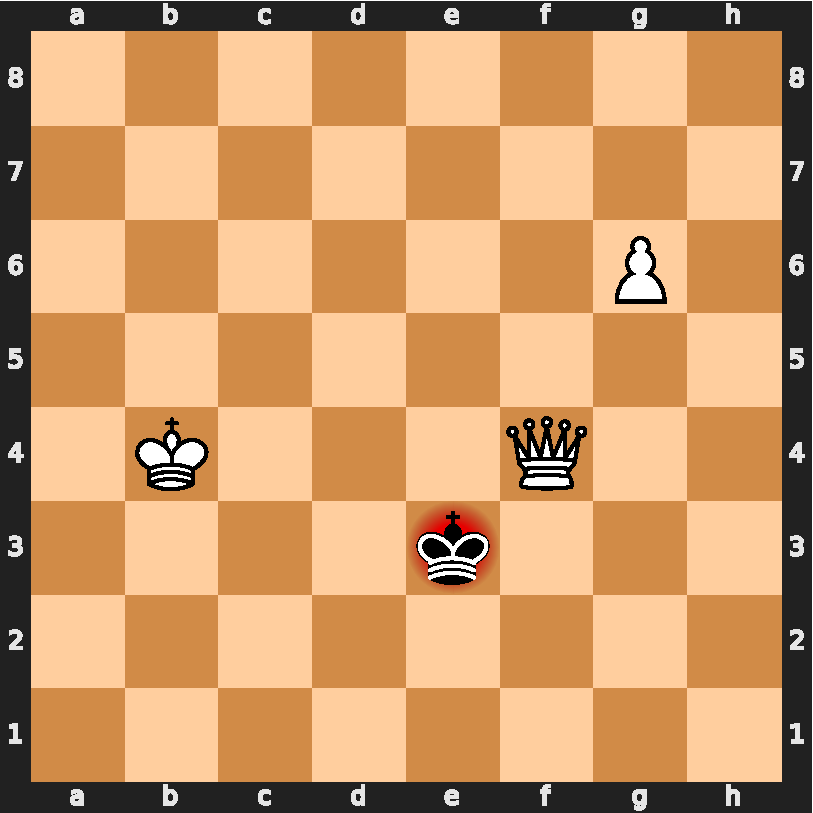
\includegraphics[width=5cm]{misplaced/pos1.pdf}
  }\\
  \subfloat[Stockfish score: -55, GAiA score: -6287]{
    \centering
    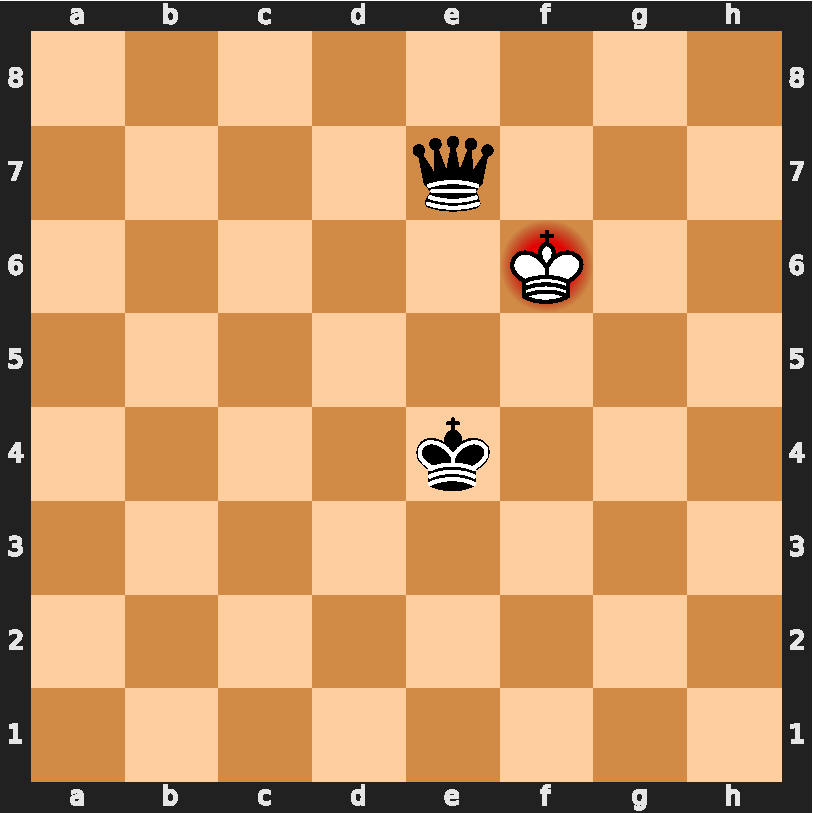
\includegraphics[width=5cm]{misplaced/pos2.pdf}
  }
  \caption{Examples of misplaced positions}
  \label{fig:misplaced}
\end{figure}

\section{Conclusion}
Artificial intelligence is being used in more and more fields.
It is becoming very complex to design models capable of answering very precise problems.
We could see through this article that it was possible (for some problems) to transform
our data into images in order to use a neural network specialized in image recognition.
It may not be the most efficient model but it allows to have very good performances easily.
In my chess example, I was able to design a chess engine able to beat any non-professional
human player in only a few hours of training. It would be interesting to find other problems
that can be solved in this way to corroborate these results.


\bibliographystyle{plain}
\bibliography{refs}


\end{document}
